\chapter{Quantum Generative Adversarial Networks}\label{chapter:quantum_gans}
The field of Quantum Machine Learning (QML) is still in very early stages and there
has been an ongoing effort on translating the  classical Machine Learning (ML)
concepts into QML realm. Because of the limitations of current quantum computers
(NISQ) \cite{bharti2021noisy} and overall different paradigm of Quantum
Computing (QC), this process is difficult and there is no clear
answer to the question ``how this concept should be realized on QC device?''.
While in classical GANs generator and discriminator are realized as deep neural
networks, NISQ devices are not yet powerful enough to support such architecture.
Instead parametric quantum circuits \cite{Schuld_2020} are used.

In this chapter we take a closer look at two different designs of quantum GANs.
We briefly explain theory behind them and show the results of our evaluation.
The quantum GANs introduced in this chapter are the base of our hybrid
classical-quantum generative framework.

\section{Standard Quantum GANs (SQGANs)}
In the classical GANs, both the discriminator and generator are deep, general
purpose neural networks. The logical extension of this design in the quantum
realm is to model those are general purpose parametric quantum circuits. This
idea was formalized by Dallaire-Demers et al. \cite{Dallaire_Demers_2018} in
the architecture we call SQGANs (Figure \ref{fig:SQGANs_circuit}). The generator
starts in the state $\ket{0}^{\otimes n}$ in the \textbf{Our R/G} wire, where
$n$ is the dimension of the real quantum samples.
Additionally, the generator takes the label state $\ket{\lambda}$ in the
\textbf{Label R/G} wire and the random state $\ket{z}$ that provides the entropy in
the \textbf{Batch R/G} wire. The label state $\ket{\lambda}$ lets the
generator to learn the conditional distribution $p_g(x|\lambda)$ instead of $p_g(x)$,
this design was inspired by classical Conditional GANs
\cite{mirza2014conditional}. The discriminator takes the generated state
$\rho_\lambda^G$ or real state $\rho_\lambda^R$ and the corresponding label
$\ket{\lambda}$ in the \textbf{Label D} wire, it also uses the workspace
\textbf{Batch D} initialized in $\ket{0}$ state. The measurement on the single
qubit wire \textbf{Out D} corresponds to the probability of the state in 
\textbf{Out R/G} being real or generated.

There are not any particular restrains on how $G$ and $D$ circuits should look
like. However, to be able to learn and differentiate between arbitrary quantum
states the ansatz used should be universal (i.e. be able to generate every
quantum state given appropriate depth). The ansatz used in this
work is described in details in Appendix \ref{apx:sqgans_ansatz}.

\begin{figure}[htbp!]
  \begin{tikzcd}
    \rstick{Out D} &&&&&& \rstick{$\ket{0}$} &&& \qw & \qw & \gate[4, disable auto height]{D(\theta_D)} & \meter{} \\
    \rstick{Batch D} &&&&&& \rstick{$\ket{0}^{\otimes d}$} &&& \qw & \qw & & \qw \\
    \rstick{Label D} &&&&&& \rstick{$\ket{\lambda}$} &&& \qw & \qw & & \qw \\ 
    \rstick{Out R/G} &&&&&& \rstick{$\ket{0}^{\otimes n}$} &&& \gate[3, disable auto height]{
      \begin{array}{c}
      R \\ or \\ G(\theta_G)
      \end{array}
    } & \qw \rho_{\lambda}^{R/G} & & \qw \\ 
    \rstick{Label R/G} &&&&&& \rstick{$\ket{\lambda}$} &&& \qw & \qw & \qw & \qw \\ 
    \rstick{Batch R/G} &&&&&& \rstick{$\ket{z}$} &&& \qw & \qw & \qw & \qw 
  \end{tikzcd}
  \caption{SQGANs schema. The discriminator $D$ and the generator $G$ are
    parametric quantum circuits. The first 3 wires go
    directly to the discriminator. \textbf{Out D} outputs the probability of the
  input being generated. \textbf{Batch D} is an additional workspace of the
  discriminator and \textbf{Label D} contains the label state. \textbf{Out R/G}
  carries the generated or real state. \textbf{Label R/G} contains the label
  state and \textbf{Batch R/G} is the noise source for the generator, not used
  with the real samples.\label{fig:SQGANs_circuit} }
\end{figure}

\subsection{Training}
As in the SGANs we are interested in the minmax game setting. Specifically, in
the \textbf{Out D} wire, the measurement of $\ket{1}$ indicates that the sample
was real and $\ket{0}$ that the state was generated by $G$.
\footnote{Using $\ket{1}$ and $\ket{0}$ in this order is just a convention we
  assume. Any other orthogonal pair can be used.}
This should be the case for each label state $\ket{\lambda}$, which gives the
objective \ref{eq:SQGANs_objective}. 
\begin{equation}
  \begin{split}
  \label{eq:SQGANs_objective}
  & \max_{D}\min_{G} \mathcal{L}(G, D) = \\
  & \max_{D}\min_{G}  \frac{1}{\Lambda}\sum_{\lambda \in \Lambda}{P((D(\theta_D, \ket{\lambda}, R(\lambda)) = \ket{1}) \land (D(\theta_D, \ket{\lambda}, G(\theta_G, \ket{\lambda}, \ket{z}) = \ket{0})))}
  \end{split}
\end{equation} 
Where the discriminator objective is to maximize the probability of measuring $\ket{1}$
given real sample and measuring $\ket{0}$ given generated state. At the same
time for the generator the objective is to do the opposite.

The SQGANs cost function \ref{eq:SQGANs_objective} in contrast to the SGANs cost
function \ref{eq:SGANs_objective} is not defined with log-likelihood. In quantum
setup is more natural to work with linear functions and since the $\log$ is
convex, the optimum is the same for both.

The cost function $\mathcal{L}(G, D)$ expressed in terms of measurements and
assuming equal probability of sampling from $R$ and $G$ takes the form \ref{eq:SQGANs_objective}

\begin{equation}
  \label{eq:SQGAN_objective_trace}
  \mathcal{L}(G, D) = \frac{1}{2} + \frac{1}{4\Lambda}\sum_{\lambda \in
  \Lambda}{}tr((\rho_\lambda^{DR}(\theta_D) - \rho_\lambda^{DG}(\theta_D, \theta_G, z))Z)
\end{equation}
For detailed derivation on how to get from \ref{eq:SQGANs_objective} to
\ref{eq:SQGANs_objective} refer to Appendix \ref{apx:sqgans_cost_function}.

\subsubsection{Gradient Estimation}
To optimize the parameters $\theta_D$ and $\theta_G$ classical gradient descent
method was used. First, the value of the cost function $\mathcal{L}(G, D)$ was
estimated by sampling from the circuit \ref{fig:SQGANs_circuit}. This allows to
calculate the gradient w.r.t. $\theta_D$ and $\theta_G$ on classical computer
and update the parameters at the step $k$ in the following way
\begin{equation}
  \begin{split}
    \theta^{k+1}_D = \theta^{k}_D + \alpha^k_D\nabla_{\theta_D}\mathcal{L}(\theta^k_G, \theta^k_D) \\
    \theta^{k+1}_G = \theta^{k}_G - \alpha^k_G\nabla_{\theta_G}\mathcal{L}(\theta^k_G, \theta^k_D)
  \end{split}
\end{equation}
where $\alpha^k_D$ and $\alpha^k_G$ are learning rate metaparameters that can
depend on the step $k$.

It is also possible to estimate the gradient directly on quantum computer by
creating an explicit quantum circuit for each element of vectors $\theta_D / \theta_G$
and reading the grading by sampling for those circuits \cite{Dallaire_Demers_2018}.
\subsection{Evaluation Results}
\subsubsection{Experimental Setup}
In all of the experiments the real samples are generated by evaluating the
circuit from Figure \ref{fig:phase_circuit_small}. This circuit was constructed
by Smith et al. \cite{smith2020crossing} to study topological phase transitions.
All the gates in the circuit are parameterized by a single real valued parameter
$g \in [-1;1]$. The detailed gates layout is described in Appendix \ref{apx:topological_phase_transition_ansatz}.
\begin{figure}[htbp!]
  \begin{tikzcd}
    \lstick{$\ket{0}$} & \gate[2, disable auto height]{U_1(g)} & \qw & \qw & \qw &
    \qw & \qw & \qw \\
    \lstick{$\ket{0}$} & & \gate[2, disable auto height]{U(g)}  & \qw & \qw & \qw & \qw & \qw \\
    \lstick{$\ket{0}$} & \qw & \qw & \gate[2, disable auto height]{U(g)}  & \qw & \qw & \qw & \qw \\
    \lstick{$\ket{0}$} & \qw & \qw & \qw & \qw & \ldots  \\
    \vdots & & & & &\ldots & \gate[2, disable auto height]{U(g)} & \qw \\
    \lstick{$\ket{0}$} & \qw & \qw & \qw & \qw & \qw & \qw & \qw \\
  \end{tikzcd}
  \caption{The circuit used for generating real samples. All the gates are
    parametrized by a real valued parameter $g \in [-1; 1]$. For detailed
    description of the circuit see Appendix
    \ref{apx:topological_phase_transition_ansatz} \label{fig:phase_circuit_small}}
\end{figure}

The generator and discriminator are both build using the generic circuit
architecture from Appendix \ref{apx:sqgans_ansatz}. The number of layers differs
and is specified for each experiment separately.

In all the experiment we use Adam optimizer \cite{kingma2017adam} with
parameters $\beta_1 = 0.9$, $\beta_2=0.98$, $\hat{\epsilon} = 1e-9$. The
learning rate is calculated as
\begin{equation}
lr = \max{(\exp{(-\frac{(k+200) * \ln{100}}{4000}), 0.01)}
\end{equation}
where $k$ is the optimization step number. The
learning rate decreases from $\sim 0.8$ to $0.01$ in the first $3800$ steps and then
remains at $0.01$ for the rest of the training. The exact values were derived
experimentally and show overall good convergence. The exact number of epochs and
iterations is specified for each experiment separately.
\subsubsection{Results For Pure State Real Input}
In this setup the generator is fed the same real input state at every iteration.
The real input state is generated using circuit from Figure
\ref{fig:phase_circuit_small} for random $g \in [-1; 1]$.


In Figure \ref{fig:sqgans_res_3} we present the
results of experiments for different widths of the real input circuit. For All
the experiments, the generator and discriminator were built using ansatz
from Appendix \ref{apx:sqgans_ansatz} for each layer. The \textbf{Label} and
\textbf{Batch} wires are not used for any circuit.

For each real input width the generator was able to approximate the real source,
increasing the fidelity as the training progressed. The training was
harder for the bigger real source circuits and it can be clearly seen that
the results for wider inputs are worse. Not only the final fidelity is lower, but
also it fluctuates much more. It is also much harder for the generator to fool
the discriminator for wider inputs.

It is not surprising that it is more difficult to train circuits with more
qubits. We also acknowledge that with different metaparameters or optimization
method the results could be better. However, our best results for more than 5 qubits
in the real source are not longer useful for the real source approximation.

\begin{figure}[htbp!]
  \captionsetup[subfigure]{labelformat=empty}
  \centering
  \subfloat{
    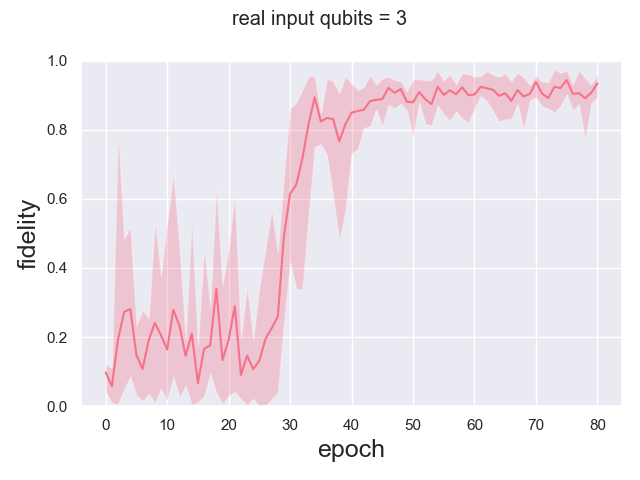
\includegraphics[width=0.3\linewidth]{figures/sqgans_size=3/fidelity.png}
  }
  \subfloat{
    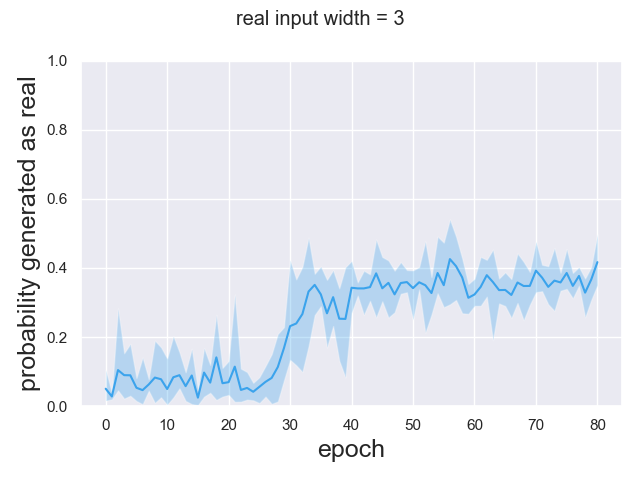
\includegraphics[width=0.3\linewidth]{figures/sqgans_size=3/probability_generated_as_real.png}
  }
  \subfloat{
    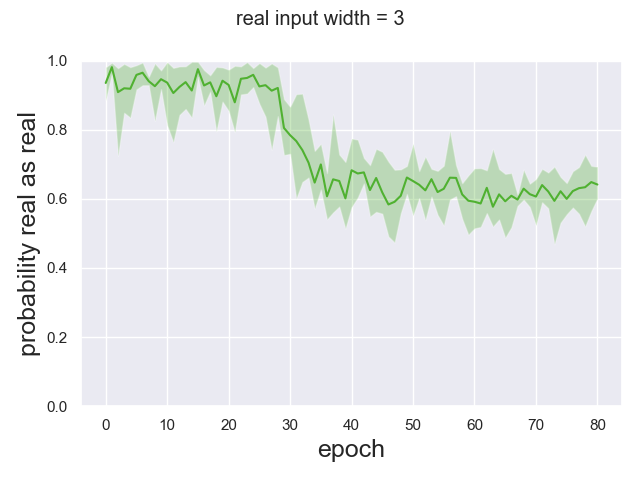
\includegraphics[width=0.3\linewidth]{figures/sqgans_size=3/probability_real_as_real.png}
  }


  \subfloat{
    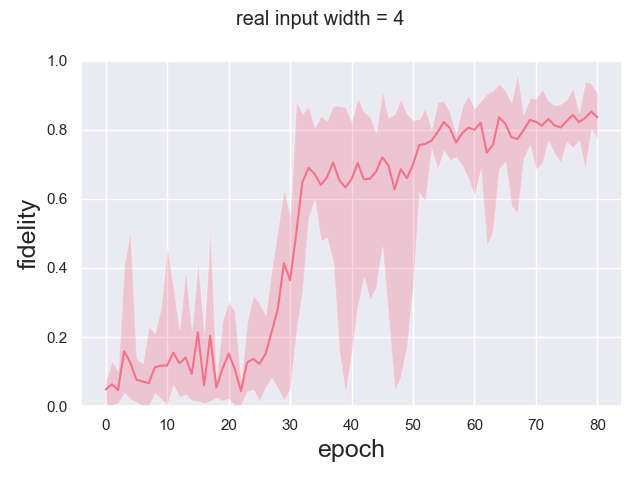
\includegraphics[width=0.3\linewidth]{figures/sqgans_size=4/fidelity.png}
  }
  \subfloat{
    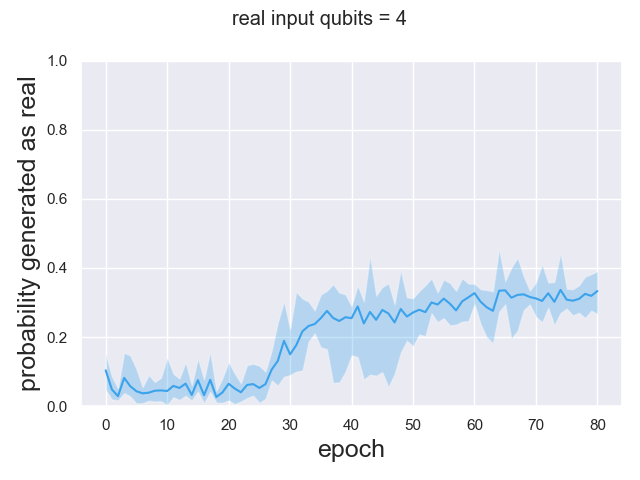
\includegraphics[width=0.3\linewidth]{figures/sqgans_size=4/probability_generated_as_real.png}
  }
  \subfloat{
    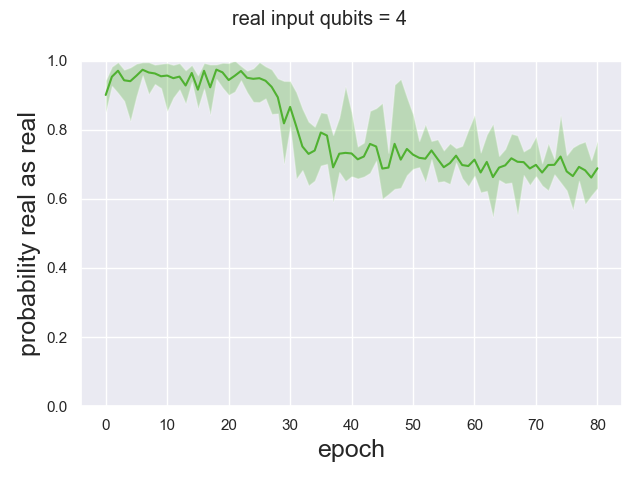
\includegraphics[width=0.3\linewidth]{figures/sqgans_size=4/probability_real_as_real.png}
  }

  \subfloat[Fidelity between real and \\generated state]{
    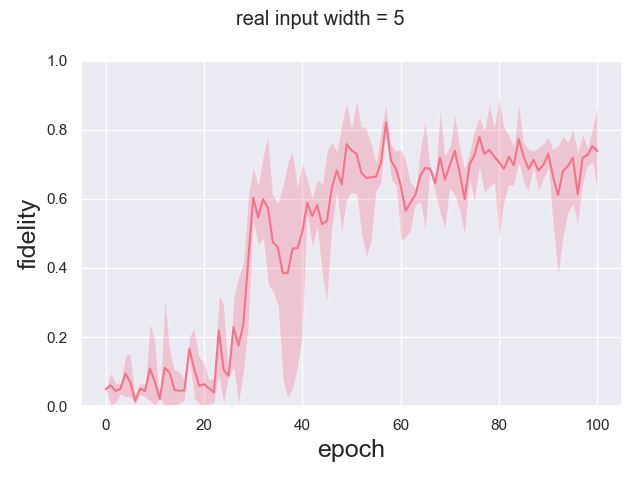
\includegraphics[width=0.3\linewidth]{figures/sqgans_size=5/fidelity.png}
  }
  \subfloat[Probability of classifying \\generated state as real]{
    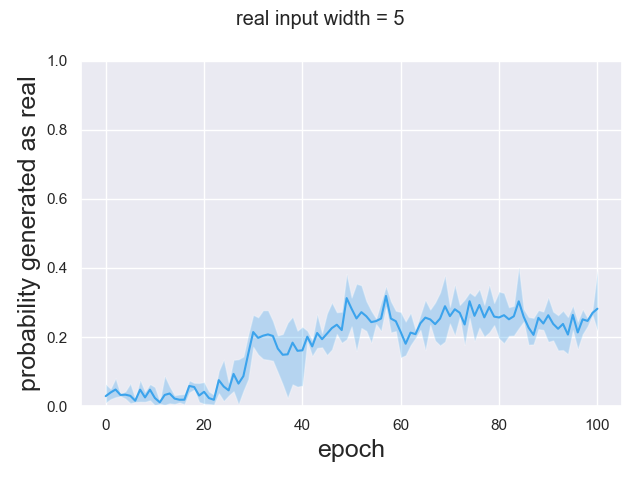
\includegraphics[width=0.3\linewidth]{figures/sqgans_size=5/probability_generated_as_real.png}
  }
  \subfloat[Probability of classifying real state as real]{
    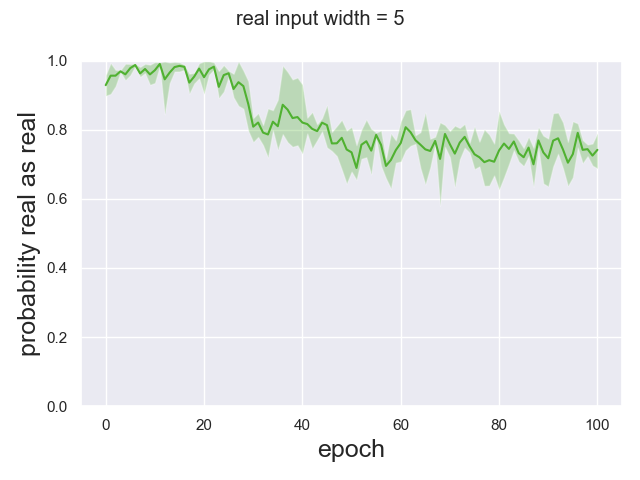
\includegraphics[width=0.3\linewidth]{figures/sqgans_size=5/probability_real_as_real.png}
  }
  \caption{The solid line represents the average value and the shaded area
    represents the range from 5 different experiments. The generator has the
    number of layers equal to the width of real input the discriminator has one
    more layer than the generator. In each epoch generator is optimized for 11 iterations and
  discriminator for 111. }
  \label{fig:sqgans_res_3}
\end{figure}
\subsubsection{Results For Mixed State Real Input}
If the real input source can provide more than one state, we can say that the
generator is learning mixed state of all the input states. Dallaire-Demers et
al. \cite{Dallaire_Demers_2018} trained a simple 2 qubits circuit with two real
input states $\ket{0}$ or $\ket{1}$. In this setup \textbf{Label} wires consist
of one qubit and also takes values $\ket{0}$ or $\ket{1}$, effectively learning
$CNOT$ gate. This strategy do not have generalize well in to more complex cases.
First, if there is more than one non-$\ket{0}$ input state, there would have to
be a separate $CNOT$ gate for each state. Second, the number of qubits necessary
for the \textbf{Label} wires grows logarithmically with the number of real input
states. Both of those cause the circuit to grow in width and depth.

Another approach we explored was to insert $R_x(\lambda_k)$ parametrized
rotation gates between each layer of the generator and discriminator. The
generator is essentially learning how to rotate input state $\ket{0}$ to some
desired real input state $\ket{r_k}$. Then, if for each $k$ the rotation is
pushed in different direction, the final generator might give different output
state for each $\lambda_k$. However, in our experiments the generator was always
learning to ignore the $R_x(\lambda_k)$ and in the end was only able to produce
one, slightly distorted, state independent of $\lambda_k$.

\subsection{Conclusions}
We have experimentally evaluated SQGANs and confirmed their ability to learn
pure quantum state. However, the problems with labeled states and small
circuit width for which the training succeeds prevented us from succeeding in
mixed state learning.

The very important aspect of generative models is ability to generate new,
unseen before, samples. In SQGANs this is theoretically possible by using the
textbf{Batch} register. However, it is not straight forward to use this register
in the intended way. First, the task of generating random quantum state is not
trivial on its own. Second, all the problems associated with the label state
$\lambda$ also apply to the random state $z$. 

Because of the above, we decided not to pursue the exploration of SQGANs further
and turned into other methods.


\section{Wasserstein Quantum GANs (WQGANs)}
  
As in the classical case, the WQGANs relay on calculating the Wasserstein
distance between real and generated state. However, the definition of the
Wasserstein distance cannot be trivially translated into the quantum setup.
There has been multiple approaches to defining the quantum Wasserstein distance
\cite{carlen2012analog,chen2016matrix,chen2018Wasserstein,ning2013matrixvalued,peyré2017quantum,golse2021quantum,Golse_2016,yu2019quantum},
however the first take on the Wasserstein distance in the context of quantum
GANs was proposed by Chakrabarti et. al\cite{chakrabarti2019quantum}. They
proposed the Wasserstein semi-metric and successfully used it to train the
quantum GANs. The shortcoming of this semi-metric is that, it does not preserve the
triangle inequality.

In this work, we use the definition by De Palma et.
al\cite{depalma2020quantum}. They proposed a generalization of
Wasserstein distance of order 1 to the quantum realm. The dual formulation of
this distance is stated as follows:
\begin{equation}
  W(\rho, \sigma) = \max_{H \in \mathcal{O}_n}{(Tr[(\rho - \sigma)H]: \norm{H}_L \leq 1
    )}
\end{equation}
Where $\mathcal{O}_n$ is a set of all $2^n \times 2^n$ Hermitian matrices.
$\norm{H}_L$ is a quantum Lipschitz constant of the matrix $H$:
\begin{equation}
  \norm{H}_L = 2 \max_{i=1\ldots n}{\min_{H_{\bar{i} \in \mathcal{O}_n}}{(\norm{H - H_{\bar{i}}}_\infty)}}
\end{equation}


%%% Local Variables:
%%% mode: latex
%%% TeX-master: "../main"
%%% End: